\section{Configuración de proyecto ejecutable: CCS}

\begin{enumerate}
    \item  Se importa el proyecto de la carpeta \textit{lab0/build} al IDE ccs entregada junto con el repositorio del curso. Una vez importado, al intentar efectuar la construcción haciendo click en \textit{build proyect} lo que se obtiene es una serie de errores y mensajes de \textit{warnings}
    
    
    Entre ellos se indica que la ruta hacia los archivos del proyecto importado, en la sección referente a la compilación, no es accesible pues indica directorios que no pertenecen al dispositivo en el que se está trabajando. Las que se indican en el proyecto inicialmente se muestran en la figura \ref{path_profe}
    
    
    \begin{figure}[H]
        \centering
        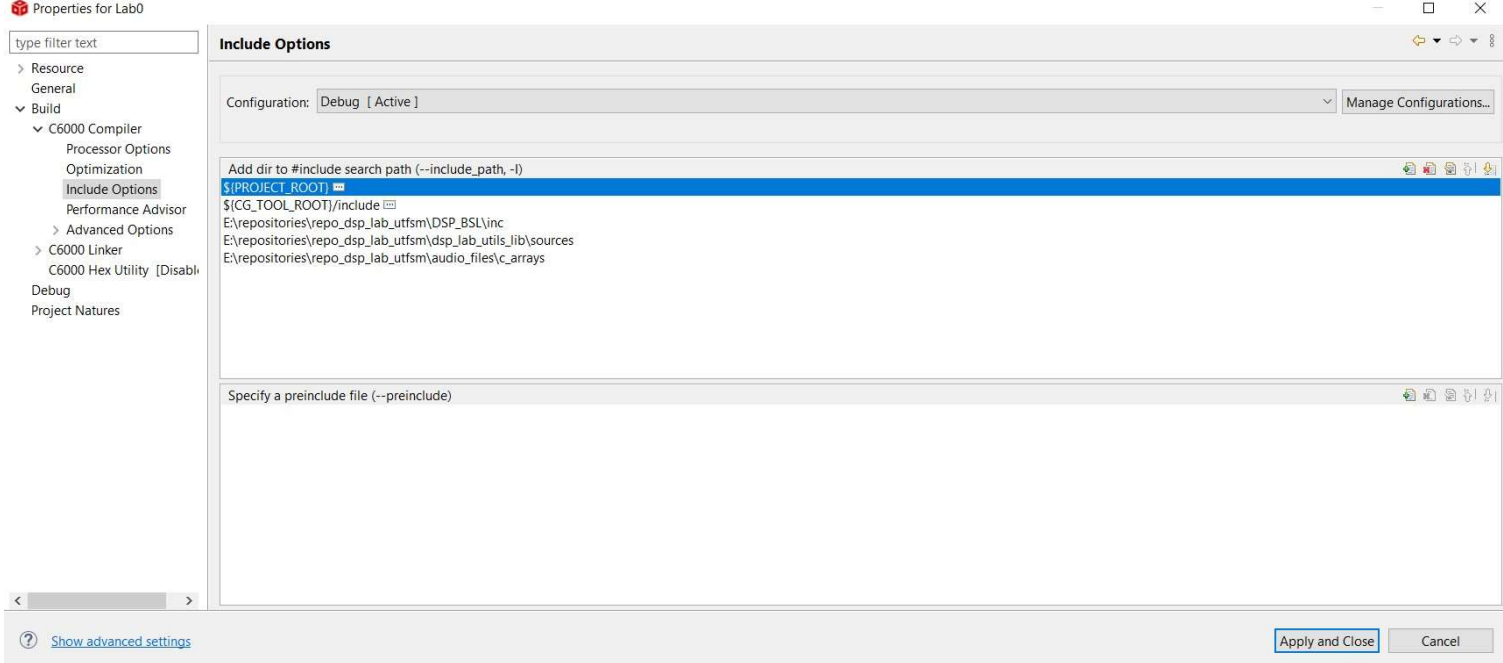
\includegraphics[width = 0.9 \linewidth]{figures/pathProfe.png}
        \caption{Configuración inicial del compilador con las rutas ajenas.}
        \label{path_profe}
    \end{figure}
    
    
    Modificando las rutas hacia la ubicación local de los archivos y añadiendo además la ruta hacia el directorio \textit{DSP\_AIC3016} , ya que también existían errores indicando que requiere archivos ubicados en ese directorio  (ver figura \ref{error}), la  sección \textit{Build C000 Linker Include Options} de configura como se muestra en la figura \ref{path_local}
    
    
    
    \begin{figure}[H]
        \centering
        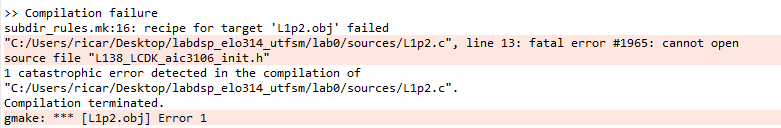
\includegraphics[scale = 0.8]{figures/error_aic3106.png}
        \caption{Error referente a la falta del directorio \textit{DSP\_AIC3016}}
        \label{error}
    \end{figure}
    \begin{figure}[H]
        \centering
        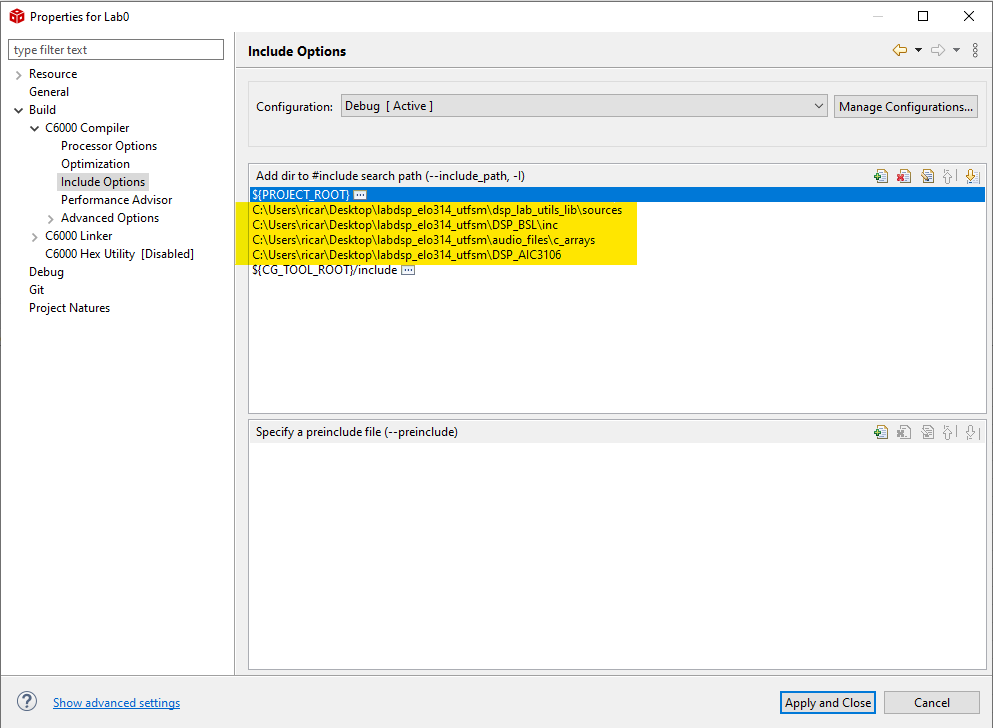
\includegraphics[scale = 0.5]{figures/path_local.png}
        \caption{Configuración del compilador con las ruta locales de trabajo.}
        \label{path_local}
    \end{figure}
    
    
    Por otro lado, se debe añadir la una dependencia extra en la sección \textit{linker}, dado que inicialmente solo se encuentra una por defecto en el proyecto, esto se muestra en la figura \ref{liker}
    
    \begin{figure}[H]
        \centering
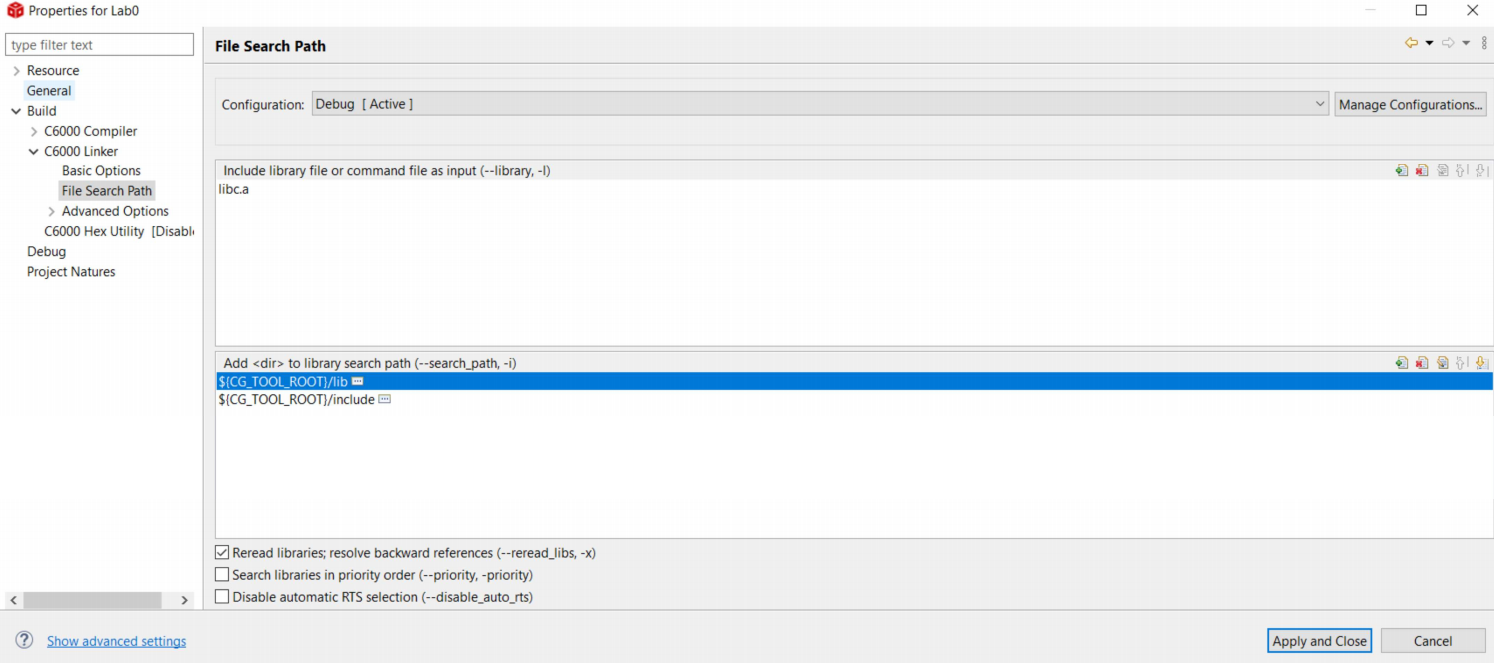
\includegraphics[scale = 0.3]{figures/linker_profe.png}
        \caption{Configuración inicial del \textit{linker} del proyecto.}
        \label{liker}
    \end{figure}
    
    
    Luego de añadir la dependencia necesaria la configuración queda de la siguiente forma
    
    \begin{figure}[H]
        \centering
        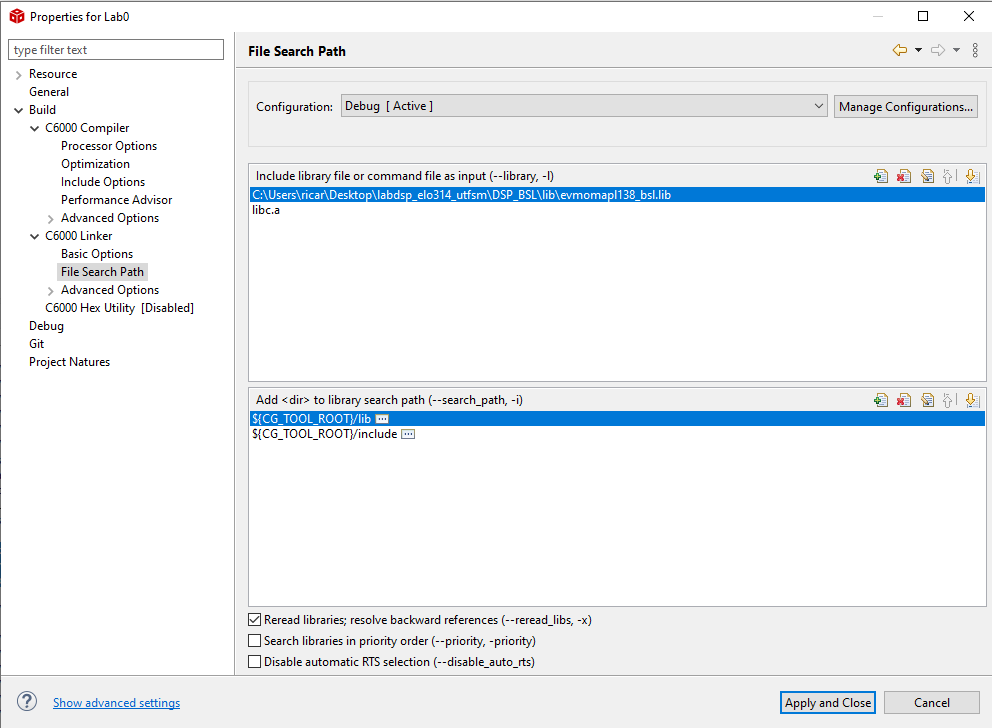
\includegraphics[scale = 0.5]{figures/linker_local.png}
        \caption{Configuración del \textit{linker} del proyecto con dependencias ya añadidas.}
        \label{fig:my_label}
    \end{figure}
    
    
    
    Para solucionar el último error que impide la construcción correcta del proyecto se añade manualmente el archivo \textit{L138\_LCDK\_aic3106\_init.c} utilizando la ruta local de dicho archivo.
    
    
    \begin{figure}[H]
        \centering
        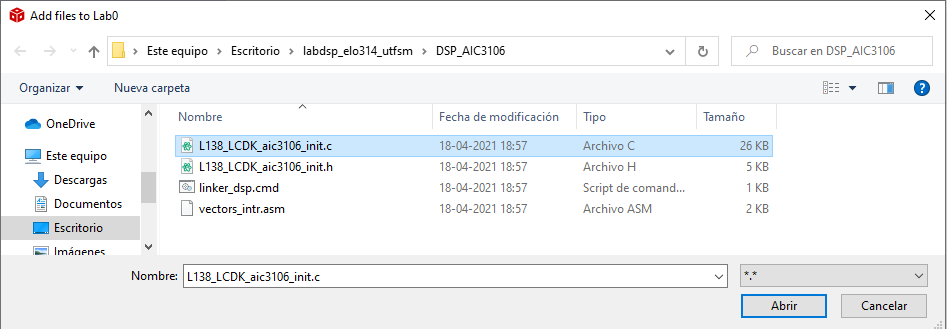
\includegraphics[scale = 0.5]{figures/aic3106.png}
        \caption{Se añade archivo \textit{L138\_LCDK\_aic3106\_init.c} requerido para construcción correcta del proyecto.}
        \label{fig:my_label}
    \end{figure}
    
    
    La figura \ref{correct_build} muestra como se ha logrado la correcta construcción del proyecto con las configuraciones hechas
    
    \begin{figure}[H]
        \centering
        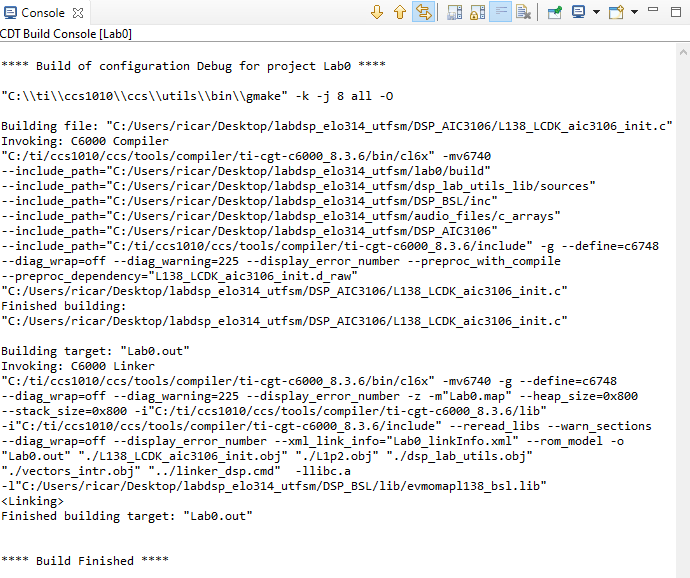
\includegraphics[scale = 0.7]{figures/correct_build.png}
        \caption{Construcción exitosa del proyecto }
        \label{correct_build}
    \end{figure}
    
    
    
\end{enumerate}